
\section{Team Collaboration}
\subsection*{Technologies}
\hfill \\
Discord was used to discuss the assignment, share each member’s progress, and discuss meeting times and locations. VS Code and Google Collaboratory were used to write the Python script, and Github was used to share the code. 
\subsection*{Management}\hfill \\
All members worked on completing the task of finding the transfer function. After that, tasks involving writing the code and the report were divided across the team. These tasks were managed well by each member and completed well on time.
\begin{figure}[ht]
    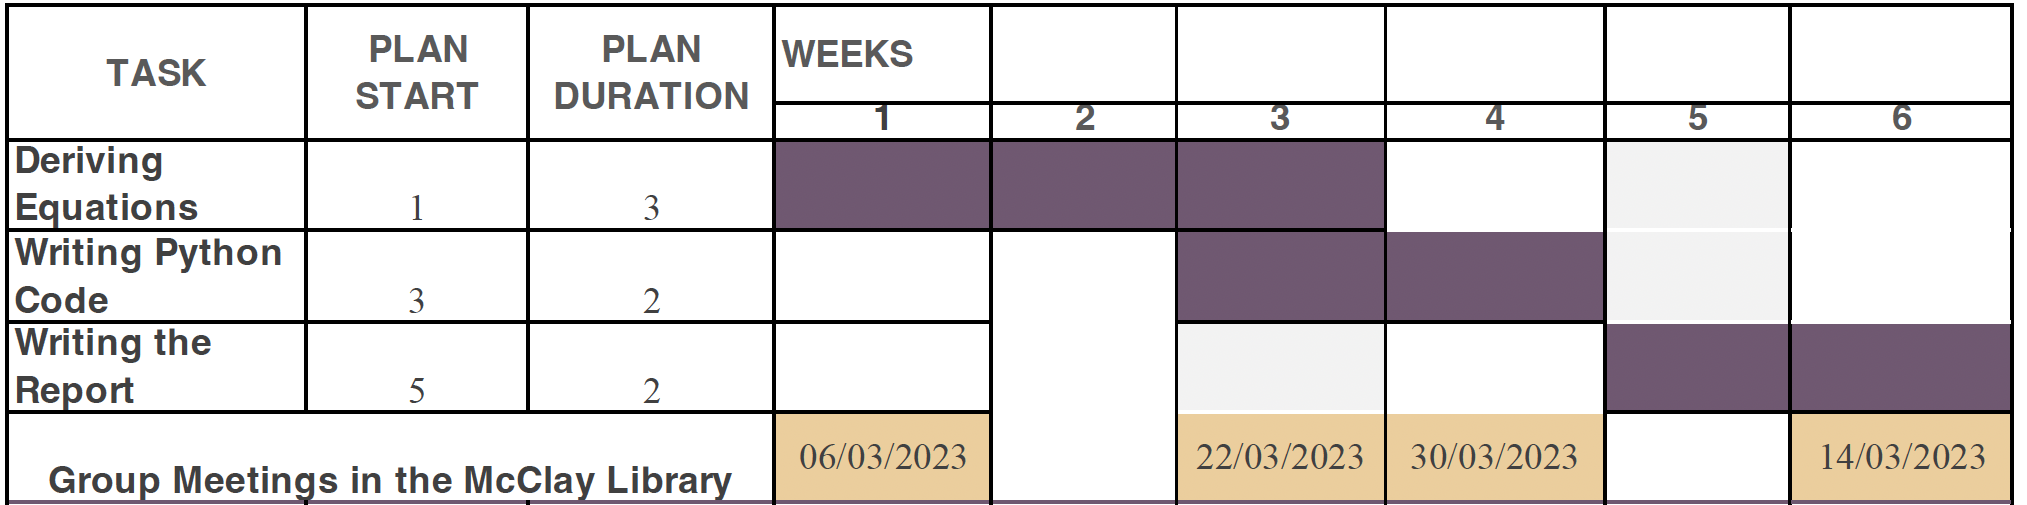
\includegraphics[width=0.8\linewidth]{Team collaboration/Screenshot 2023-04-16 at 19.28.44.png}
    \caption{Gantt chart of time management for coursework}
\end{figure}
\subsection*{Challenges}\hfill \\
Deriving the transfer function was a big challenge we faced and spent most of our time on.  
Choosing the PID values became a challenge as we tried to find the values that gave the best output. The values were decided using trial and error until we found values that we found to be good 
\subsection*{Contributions}\hfill \\
Each team member individually worked on deriving the equations and shared their progress with the other team members for them to compare and check the results.
\\
The tasks involving Python were divided as follows:
\begin{itemize}
  \item Michael Loughran worked on writing the code and the LaTeX for the equations, including the modelling of the system and the transfer function.
  \item Xiaohan Song worked on writing the code and the LaTeX for the simulations of the controller.
  \item Scott McNeilly worked on writing the bulk of the report and combining the sections of the other team members into one final report.
\end{itemize}
